\subsection{ATAC-sequencing and CTCF sequencing}
When studying chromatin, it is often very interesting to know where it is more open and accessible, and where the CTCF bins to the structure. To know these information, it is possible to perform ATAC-sequencing and CTCF ChIP-sequencing, respectively. Below it is reported a brief description of the two methods:

\begin{itemize}
  \item \textbf{ATAC-sequencing} is a technology that allows for the identification of open chromatin regions 
  \cite{buenrostroTranspositionNativeChromatin2013a, grandiChromatinAccessibilityProfiling2022}. 
  In order to work, it requires the addition of TN-5, a hyper-active transposase. The latter is preloaded with sequencing adapters
  \cite{grandiChromatinAccessibilityProfiling2022}
  to induce a contempourary reaction of fragmentation and ligation of the pieces released, in a process called segmentation. The obtained adapted fragments are then amplified and sequenced. Once the reads are generated, a peak-calling algorithm (generally MACS-2 
  \cite{zhangModelbasedAnalysisChIPSeq2008a}) 
  is used to determine which portions of the genome present ATAC peaks, and areas where there are significant enrichments of aligned reads with respect to the background. A significant enrichment of reads is possible only in accessible regions, which are generally also the most active ones and with available sites for transcription factors binding.
  \item The \textbf{CTCF Chip-sequencing} data used for this experiment, named in table \ref{tab:data}, were obtained through a classical procedure: it consisted on combining a process of chromatin immunoprecipitation, made wiith antibodies specific for CTCF, and one of DNA sequencing
  \cite{shahChromatinImmunoprecipitationSequencing2009}. 
  The scope of the technique is to infer the possible binding sites of the transcription factor on the DNA.
  
\end{itemize}

\noindent More details about the used data can be found by consulting the ENCODE
\cite{encodeprojectconsortiumIntegratedEncyclopediaDNA2012}
 entries written in table \ref{tab:data}.

\begin{figure}[H]
    \centering
    
    \begin{subfigure}{\textwidth}
      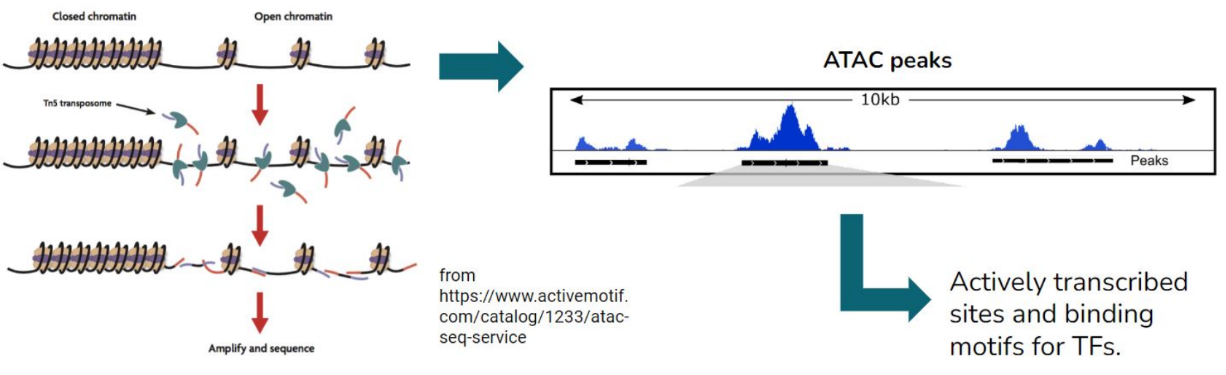
\includegraphics[width=0.95\linewidth]{./ATAC_sequencing.png}
      \caption{Basic concept behind the ATAC-sequencing technique. The images on the left and on top were taken from the following \href{https://www.activemotif.com/catalog/1233/atac-seq-service}{link}
      \cite{ATACSeqServicesEndtoEnd}.}
      \label{fig: ATAC-sequencing}
    \end{subfigure}
    \hfill
    \begin{subfigure}{0.50\textwidth}
      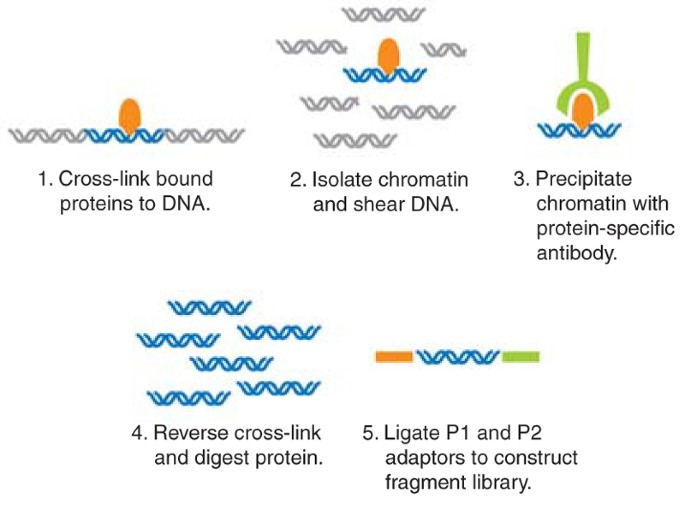
\includegraphics[width=\linewidth]{./ChIP-Seq_procedure.png}
      \caption{Pipeline to perform a generic ChIP-sequencing analysis. The image was taken from the work of Anjali Shah\cite{shahChromatinImmunoprecipitationSequencing2009}.}
      \label{fig: CTCF ChIP-Seq}
    \end{subfigure}
  
    \caption{The ATAC and CTCF procedures explanations.}
    % \label{fig:}
\end{figure}

Very interestingly, chromatin portions can be associated to a finite number of states, called chromatin states, on the base of the epigenetic data they produce
\cite{ernstChromatinstateDiscoveryGenome2017}. 
Some machine learning approaches, like \textit{ChromHMM}
\cite{chilledhousevibesLearningChromatinStates2015} 
were built with the intention of predicting these configurations. The next chapter (\ref{intro: chromhmm}) will talk about that.